%----------------------------------------------------------------------------
\chapter{Models}\label{sect:Models}
%----------------------------------------------------------------------------
In this chapter I will introduce the models I experimented with. Encode Process Decode model has been defined in the graph\_nets demos. The SimpleGraphAttention and the GraphAttention models are defined by me.

\section{Encode Process Decode model}
This model has been tested and used in the demos provided on \href{https://github.com/deepmind/graph_nets/blob/master/graph_nets/demos/models.py}{GitHub}\footnote{\url{https://github.com/deepmind/graph_nets/blob/master/graph_nets/demos/models.py}}.
\begin{figure}[!ht]
	\centering
	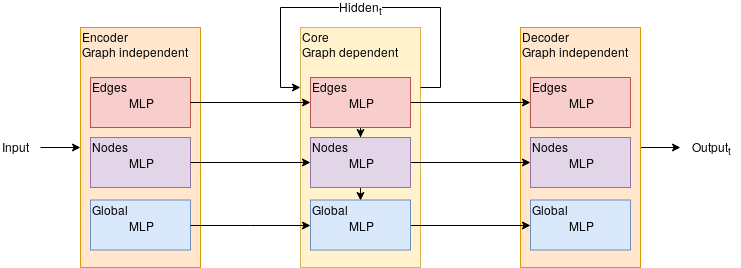
\includegraphics[width=150mm, keepaspectratio]{figures/EPD.png}
	\caption{Representation of the model.}
	\label{fig:encode-process-decode}
\end{figure}

As it is shown on the Figure~\ref{fig:encode-process-decode} above the model consist of 3 different parts.

\subsection{Encoder}
The encoder model is a graph independent model that uses multi layer perceptrons and layer normalization on the global attributes, the edge feature vectors and the node feature vectors. There are no shared variables between the multi layer perceptrons.

\subsection{Core}
This is the only graph dependent part of the model. It also uses multi layer perceptrons and layer normalization as the previous one, but the graph dependency enables it to use the predicted edge features to influence the node features and these impact the global feature.

This section of the network is repeated resulting in a hidden state that gets feed forward again in the Core section. Each step has its own output with its timestamp.

\subsection{Decoder}
The decoder model has the same structure as the encoder. It does not use any kind of activation on the last layer, which enables it to better generalize, but also making it harder to use on a specific project eq. classifying whether or not the summary graph contains the given node or edge.

\section{SimpleGraphAttention model}
I based the architecture of this model on the Encode Process Decode model. I modified it to be better suited for NLP problems, because it transforms the input words into higher dimension vector space, as you can see on Figure~\ref{fig:graph-attention0}.

\begin{figure}[!ht]
	\centering
	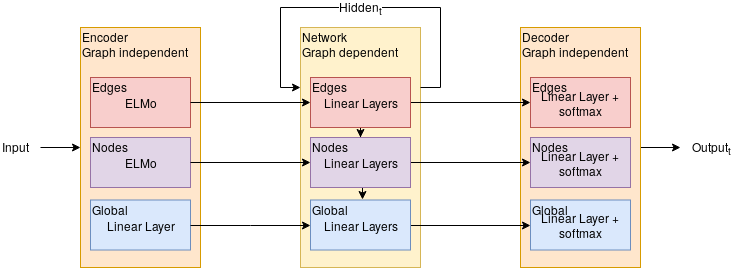
\includegraphics[width=150mm, keepaspectratio]{figures/GA0.png}
	\caption{Representation of the model.}
	\label{fig:graph-attention0}
\end{figure}

\subsection{Encoder}

The encoder part of the network contains two Embedding layers; one for the lemmas of the nodes and one for the edges' type (See Figure~\ref{fig:graph-attention0-encoder}). 

\begin{figure}[!ht]
	\centering
	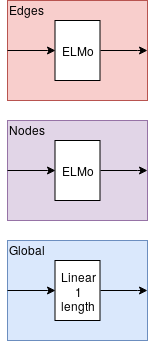
\includegraphics[scale=0.5]{figures/GA0_encoder.png}
	\caption{Representation of the encoder part of the model.}
	\label{fig:graph-attention0-encoder}
\end{figure}

The second one's necessity is questionable, since it does not contain as much information and could be also represented with a simple one-hot encoded vector, since it has not as high dimensionality as the nodes. However I decided I leave it in the model and make it a changeable parameter of the network.

For the global features I only used a simple linear layer without activation functions, since it does not need to be encoded in any way. All of these blocks work independently from each other, updating their respective blocks, because the parts are defined as the edge, node and global functions for a GraphIndependent block.

\subsection{Network}

The Network, or core part of the model consists of activated linear layers with differing sizes as depicted on Figure~\ref{fig:graph-attention0-network}.

\begin{figure}[!ht]
	\centering
	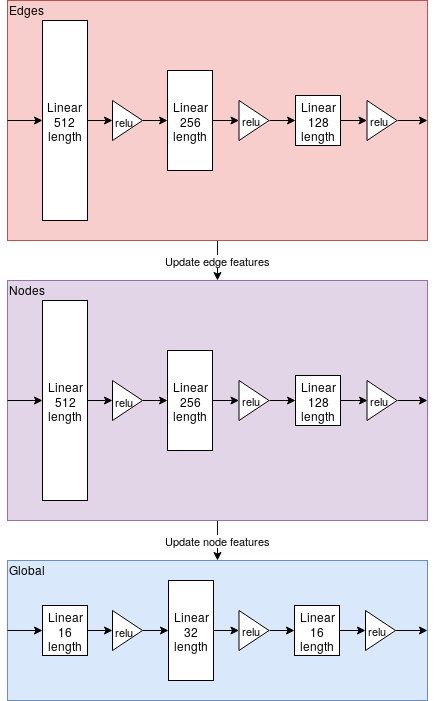
\includegraphics[scale=0.5]{figures/GA0_network.png}
	\caption{Representation of the network part of the model.}
	\label{fig:graph-attention0-network}
\end{figure}

Since this section of the model is graph dependent, after each feature update, the next block gets the updated feature vectors instead of the original ones.

\subsection{Decoder}

The decoder part of the model is also graph independent just like the encoder and it simply serves the function of the softmax output of the whole network. Its structure is presented on Figure~\ref{fig:graph-attention0-decoder}.

\begin{figure}[!ht]
	\centering
	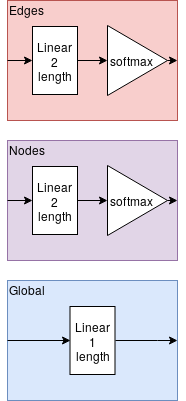
\includegraphics[scale=0.5]{figures/GA0_decoder.png}
	\caption{Representation of the decoder part of the model.}
	\label{fig:graph-attention0-decoder}
\end{figure}

\section{GraphAttention model}
The starting point of this model was the \textit{SimpleGraphAttention} model which I further developed using recent advancements regarding attention in graphs. There was two versions of this model, one that used LSTM cells in the Network part in the node block, and the other that used only linear layers. Since the main structure is the same I only included the graphical presentation on Figure~\ref{fig:graph-attention1} and Figure~\ref{fig:graph-attention1-network} of the later version. This one proved to be more usable due to the large amount of memory usage of the LSTM cells.

\begin{figure}[!ht]
	\centering
	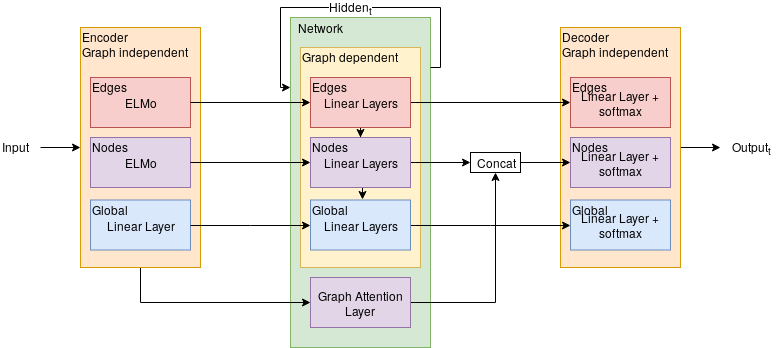
\includegraphics[width=150mm, keepaspectratio]{figures/GA1.png}
	\caption{Representation of the model.}
	\label{fig:graph-attention1}
\end{figure}


The Encoder and Decoder segments of the network are identical to their correspondences in the SimpleGraphAttention model.

\subsection{Network and Graph Attentional Layer}
The network part of the model went under some changes compared to the SimpleGraphAttention model's Network. The most notable change is the new, independent part of the network, called GAT. You can see a simplification of the network on Figure~\ref{fig:graph-attention1-network}.

\begin{figure}[!ht]
	\centering
	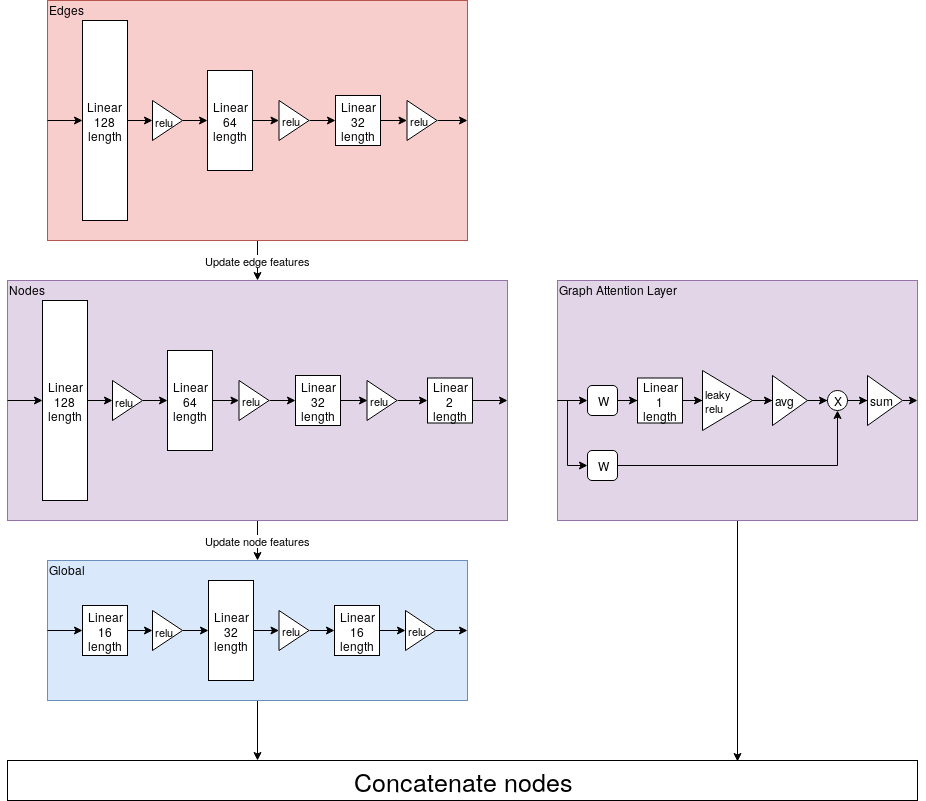
\includegraphics[scale=0.5]{figures/GA1_network.png}
	\caption{Representation of the network part of the model.}
	\label{fig:graph-attention1-network}
\end{figure}

The Graph Attentional Layer has been described in a 2018 paper titled \textit{Graph Attention Networks}~\cite{GAT}. It was designed to work well with Graph Convolutional Network structures, but I was able to implement it for the Graph Neural Network architecture as well.

This layer updates node features the following way: Suppose the features of the nodes are \(h_i\), we define a weight matrix \(W \in \mathbb{R}^{input\ features} \times \mathbb{R}^{output\ features} \) and a feed forward attention layer.

Let the normalized attention coefficients be:

\[a_{ij} =  \frac{exp(LeakyReLU(attention(W\vec{h_i} || W\vec{h_j})))}{\sum_{k \in i\ neighbors} exp(LeakyReLU(attention(W\vec{h_i} || W\vec{h_k})))}\]
if i and j are neighbors.

\[\vec{h_i}' = \sigma(\sum_{j \in i\ neighbours}a_{ij}W\vec{h_j})\]

Since we are working with multi-head attention, the update equation is modified as follows:
\[\vec{h_i}' = \sigma(\frac{1}{K} \sum_{k=1}^{K}\sum_{j \in i\ neighbours}a_{ij}^kW^k\vec{h_j})\]

Where K is the number of heads in the multi-head attention.
